\chapter{LASER: Light Amplification by Stimulated Emission of Radiation}
\graphicspath{{./cap_1/images/}}

\section*{Concetti introduttivi}

\begin{description}
    \item [Fotone:]  quanto di energia dell'onda elettromagnetica. In assenza di onde e.m. si ha comunque rumore quantistico ovvero energia di punto zero;
    \item [Assorbimento:] cancellazione di un fotone e eccitazione di un elettrone;
    \item [Emissione stimolata:] decadimento di un elettrone e creazione di un fotone a causa di un ulteriore fotone. Il fotone generato è clone del fotone generante. Essi sono quindi indistinguibili fra di loro;
    \item [Emissione spontanea:] in assenza di perturbazione (ad esclusione del rumore quantistico) l'elettrone decade emettendo un fotone.
\end{description}

\section{Processi elementari di interazione radiazione-materia}

\begin{wrapfigure}{R}{0.3\textwidth}
    \centering
    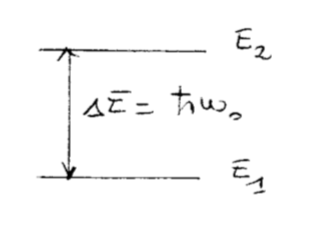
\includegraphics[width=0.9\linewidth]{jump}
\end{wrapfigure}

Consideriamo una collezione di atomi a due livelli di energia:  chiamiamo $E_1$ il primo livello, il quale è tipicamente il livello fondamentale dell'atomo, e $E_2 > E_1$ il secondo, che rappresenta lo stato eccitato con frequenza di risonanza:
\begin{equation*}
    \omega_0 \equiv \frac{E_2 - E_1}{\hbar}
\end{equation*}

Siano $N_1$ e $N_2$ le popolazioni atomiche, ovvero il numero di atomi per unità di volume sui livelli \lv{1} e \lv{2}. Si consideri poi un'onda e.m. monocromatica di frequenza $\omega$ che incide sulla collezione di atomi.\\
\\
Distinguiamo le varie casistiche.

\subsection{Assorbimento}

Qualitativamente il processo di assorbimento popola $N_2$ secondo la relazione:
\begin{equation*}
    \left( \frac{dN_2}{dt} \right)_{assorb.} = W_{12} N_1
\end{equation*}

\begin{wrapfigure}{R}{0.3\textwidth}
    \centering
    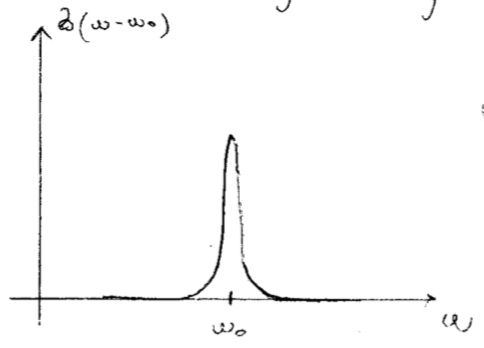
\includegraphics[width=0.9\linewidth]{deltad}
\end{wrapfigure}

dove, secondo la teoria semi-classica, il rate di assorbimento $W_{12}$ vale $W_{12} = \frac{I}{\hbar\omega} \cdot \sigma_{12}(\omega - \omega_0) = F \cdot \sigma_{12}(\omega - \omega_0)$ con $I$ l'intensità dell'onda incidente, $F = \frac{I}{\hbar\omega}$ il flusso fotonico e $\sigma_{12}(\omega -\omega_0)$ la \textit{cross-section} d'assorbimento della transizione \lv{1} $\leftrightarrow$ \lv{2} centrata in $\omega_0$.

La teoria semi-classica consente il calcolo di $\sigma_{12}$, la quale è quasi una delta di Dirac $\delta(\omega - \omega_0)$, cioè il processo di assorbimento di radiazione e.m. da parte di un atomo è un processo risonante il quale avviene solo se $\omega \approx \omega_0$. Ciò è giustificabile perché il processo di assorbimento deve conservare l'energia totale.

\subsection{Emissione stimolata}
\begin{wrapfigure}{R}{0.3\textwidth}
    \centering
    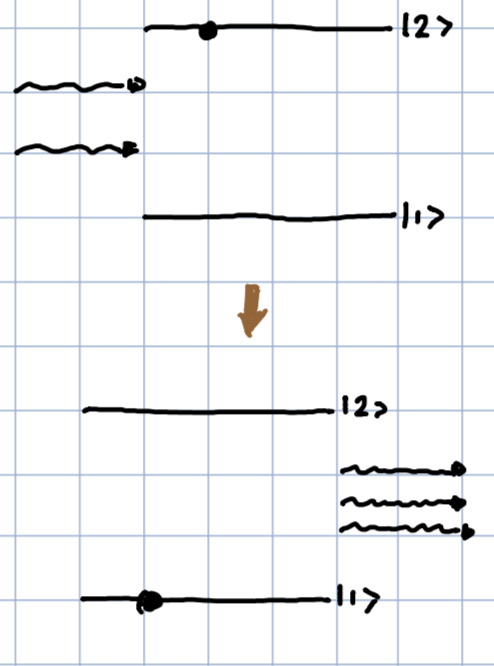
\includegraphics[width=0.9\linewidth]{emiss_stim}
    \caption{Emissione stimolata.}
\end{wrapfigure}

Un atomo nel livello \lv{2} che vede passare un fotone della giusta frequenza decade nel livello \lv{1} emettendo radiazione. Si crea un fotone identico: stesso modo, stessa frequenza, stessa polarizzazione etc. In tal caso possiamo scrivere secondo la teoria semi-classica:
\begin{equation*}
    \left( \frac{dN_2}{dt} \right) = W_{21} N_2
\end{equation*}

dove $W_{21} \equiv F \sigma_{21}(\omega - \omega_0)$.
Si dimostra che $W_{21} = W_{12}$ e quindi che $\sigma_{12} = \sigma_{21}$.\\

Cosa accade se su un atomo della popolazione $N_2$ non incide nessuna onda? Ci sono 2 possibilità.

\subsection{Emissione spontanea}

Un atomo inizialmente su \lv{2} in assenza di onde e.m. incidenti, spontaneamente, tende a decadere sul livello \lv{1}. Il modo spaziale, stato di polarizzazione, etc. del fotone emesso per emissione spontanea è casuale.\\
In tal caso:
\begin{equation*}
\left( \frac{dN_2}{dt} \right)_{\substack{emiss.\\ spont.}} = -\frac{N_2}{\tau_{spont.}}
\end{equation*}
con $\tau_{sp}$ si indica il tempo di vita \textit{radiativo} del livello eccitato \lv{2}.\\
Il decadimento nello spazio radiativo vuoto è dovuto alle fluttuazioni di energia di punto zero.

\subsection{Decadimento non-radiativo}

Un atomo in stato eccitato può decadere su un livello energetico inferiore mediante processi collisionali con altri atomi, senza emissione di fotone. L'energia interna dell'atomo può essere trasferita al partner urtante come energia cinetica (collisioni super elastiche), ceduto come energia interna oppure come ceduto ai fononi reticolari (nei solidi).\\
\\
Generalmente scriviamo:
\begin{equation*}
    \frac{dN_2}{dt} = - \frac{N_2}{\tau_{\text{non rad.}}}
\end{equation*}
dove $\tau_{\text{non rad.}}$ è il tempo di vita \textit{non radiativo} del livello eccitato \lv{2}.

\section{Assorbimento e amplificazione della luce}

Si consideri un'onda piana monocromatica di frequenza $\omega$ che si propaga in un mezzo materiale costituito da una collezione di atomi a due livelli.

\begin{wrapfigure}{R}{0.4\textwidth}
    \centering
    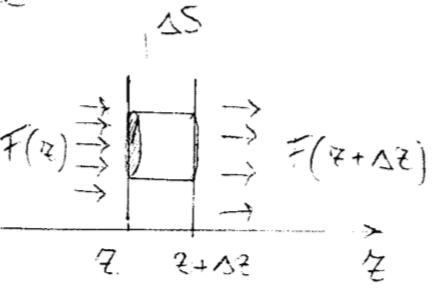
\includegraphics[width=0.9\linewidth]{flux}
\end{wrapfigure}

Siano $I(z)$, e $I(z + \Delta z)$ rispettivamente le intensità dell'onda in $z = z_0$ e $z = z_0 + \Delta z$.\\
Nel volume $\Delta V = \Delta S \Delta z$ si ha che il numero di fotoni distrutti nel volume $\Delta V$ nell'intervallo di tempo $\Delta t$ è pari a:
\begin{equation*}
    W_{12} N_1 \Delta V \Delta t
\end{equation*}
e che il numero di fotoni creati nel volume $\Delta V$ nell'intervallo di tempo $\Delta t$ è:
\begin{equation*}
    W_{21} N_2 \Delta V \Delta t
\end{equation*}

Deve quindi valere il seguente bilancio fotonico:
\begin{equation*}
    F(z + \Delta z) \Delta S \Delta t - F(z) \Delta S \Delta t = \underbrace{W_{12} N_1 \Delta V \Delta t}_\text{emissione stimolata} - \underbrace{W_{21} N_2 \Delta V \Delta t}_\text{assorbimento}
\end{equation*}

Siccome $W_{12} = W_{21} = \sigma(\omega - \omega_0) F$ si ha:
\begin{equation*}
    F(z + \Delta z) \Delta S \Delta t - F(z) \Delta S \Delta t = \sigma F(N_2 - N_1) \Delta z
\end{equation*}

quindi al limite per $\Delta z \rightarrow 0$:
\begin{equation*}
    \frac{dF}{dz} = \sigma \Delta N F \quad \text{con} \quad \Delta N \equiv N_2 - N_1 \quad \text{detta inversione di popolazione}
\end{equation*}

Dato che $F = \frac{I}{\hbar \omega}$ allora si ha che $\frac{dI}{dz} = \s \D N I$.\\
Supponendo $\Delta N$ indipendente da $z$ e da $I$\footnote{In generale non è vero a causa del fenomeno di saturazione.} si ha:
\begin{equation*}
    I(z) = I(0) e^{\sigma \Delta N z}
\end{equation*}

Distinguiamo due casi:

\begin{itemize}
    \item $N_1 > N_2$ cioè $\Delta N < 0$. Posto $\alpha \equiv (N_1 - N_2) \sigma$, il coefficiente di assorbimento del materiale, si ha:
    \begin{equation*}
        I(z) = I(0) e^{-\alpha z}
    \end{equation*}
    In questo caso, il mezzo è un assorbitore.
    \item $N_1 < N_2$ cioè $\Delta N > 0$. Posto $g \equiv (N_2 - N_1) \sigma$, il coefficiente di guadagno del materiale, si ha:
    \begin{equation*}
        I(z) = I(0) e^{g z}
    \end{equation*}
    In questo caso il mezzo è un amplificatore di luce.
\end{itemize}

Si noti che, all'equilibrio termodinamico a temperatura T, la distribuzione delle popolazioni atomiche è dato dalla distribuzione di Boltzmann:
\begin{equation*}
    \frac{N_2}{N_1} = e^{-\frac{E_2 - E_1}{k_B T}} = e^{-\frac{\hbar \omega_0}{k_B T}} < 1
\end{equation*}

Si tratta del caso $N_1 > N_2$ per cui non c'è inversione di popolazione. Per ottenere un amplificatore di luce si deve destabilizzare la distribuzione delle popolazioni con un meccanismo detto di \textit{pompaggio}. Generalmente, nei laser, si tratta di pompaggio elettrico oppure ottico.

\section{Principi e funzionamenti del laser}
Schema di un laser:
\begin{figure}[H]
    \centering
    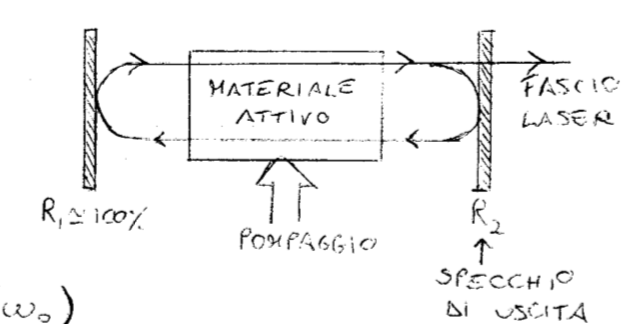
\includegraphics{schema_laser}
\end{figure}
dove indichiamo con $R_1$ e $R_2$ rispettivamente le riflettività degli specchi e con $l$ le dimensioni della cavità.\\
\\
Consideriamo un certo numero di fotoni nella cavità emessi per emissione spontanea.\\
Sia $F_1$ il flusso fotonico iniziale 
Nei successivi pompaggi all'interno della cavità il flusso fotonico si modifica così:
\begin{align*}
    & F_2 = F_1 e^{gl} \quad \text{con} \quad g \equiv (N_2 - N_1) \sigma = \sigma \Delta N\\
    & F_3 = R_2 F_2 = R_2 F_1 e^{gl}\\
    & F_4 = F_3 e^{gl} = R_2 F_1 e^{2gl}\\
    & F_5 = R_1 F_4 = R_1 R_2 F_1 e^{2gl}
\end{align*}

Introdotte le perdite logaritmiche $\gamma$ del risonatore:
\begin{equation*}
    \gamma \equiv -\frac{1}{2} \left[\ln (R_1) + \ln (R_2) \right] \qquad \rightarrow \qquad R_1 R_2 = e^{-2 \gamma}
\end{equation*}

si ha:
\begin{equation*}
    F_5 = F_1 e^{2(gl - \gamma)}
\end{equation*}

Quanto appena detto è valido per un \textit{round trip}.

\begin{figure}[H]
    \centering
    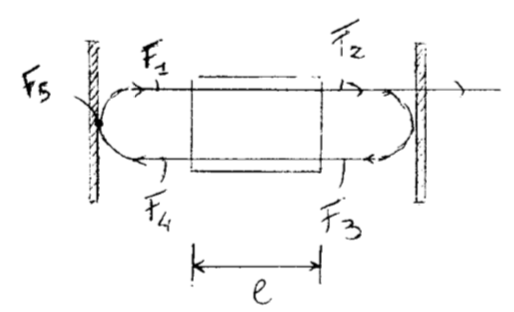
\includegraphics[width=10cm, height=4cm]{flux_schema_laser}
\end{figure}

All'n-esimo round trip si ha evidentemente:

\begin{equation*}
    F^{(n)} = F^{(0)} e^{2n(gl - \gamma)} \qquad n = 1, 2, 3, ...
\end{equation*}

Si distinguano quindi due casi:
\begin{itemize}
    \item laser \textbf{sotto-soglia} ($\gamma > gl$)\\
    Se $\gamma > gl$ allora $\gamma > \s \D N l$ e quindi $\D N < \frac{\gamma}{\sigma l}$ e $F^{(n)} \rightarrow 0$ ovvero il fotone emesso per emissione spontanea non riesce ad innescare la reazione a catena in cavità.
    \item laser \textbf{sopra-soglia} ($\gamma \leq gl$)\\
    Se $\gamma \leq gl$ allora $\D N > \s \D N_{th}$ dove per definizione $\D N_{th} \equiv \frac{\gamma}{\s l}$ detta \textit{inversione di popolazione critica} o di soglia.
\end{itemize}

\section{Meccanismo di pompaggio}

\subsection{Laser a due livelli}

\begin{figure}[H]
    \centering
    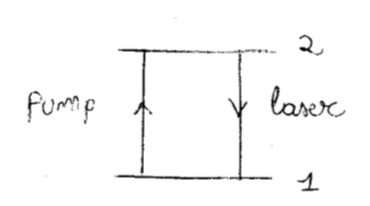
\includegraphics[width=4cm]{due_livelli}
\end{figure}

Questo tipo di laser non funziona. Al massimo si possono ottenere con metodi di pompaggio convenzionali $N_2 \leq N_1$ (trasparenza $N_2 = N_1$) ma mai $N_2 > N_1$

\subsection{Laser a tre livelli}

\begin{figure}[H]
    \centering
    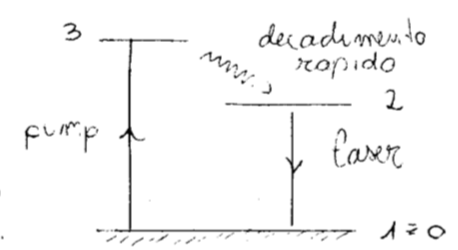
\includegraphics[width=4cm]{tre_livelli}
\end{figure}

Questo tipo di laser invece funziona ma non è ottimale, infatti per avere inversione di popolazione serve invertire più della metà degli atomi.

\subsection{Laser a quattro livelli}

\begin{figure}[H]
    \centering
    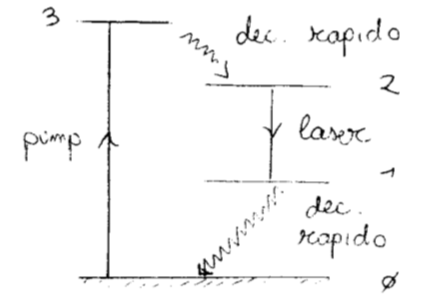
\includegraphics[width=4cm]{quattro_livelli}
\end{figure}

Questa è la soluzione ottimale perché è sufficiente invertire solo un atomo per avere inversione di popolazione.

\section{Proprietà della luce laser}

\begin{itemize}
    \item coerenza temporale (monocromaticità)
    \item coerenza spaziale
    \item direzionalità
    \item brillanza
    \item generazione di impulsi brevi
\end{itemize}